\section{Day 18}
\begin{tabular}{|c|c|}
\hline
Date: & 24.10.2013 \\
\hline
\end{tabular}
\subsection{Presented our idea to Randy}
Our idea was to make a webapp that will cover Randys requirements.\\
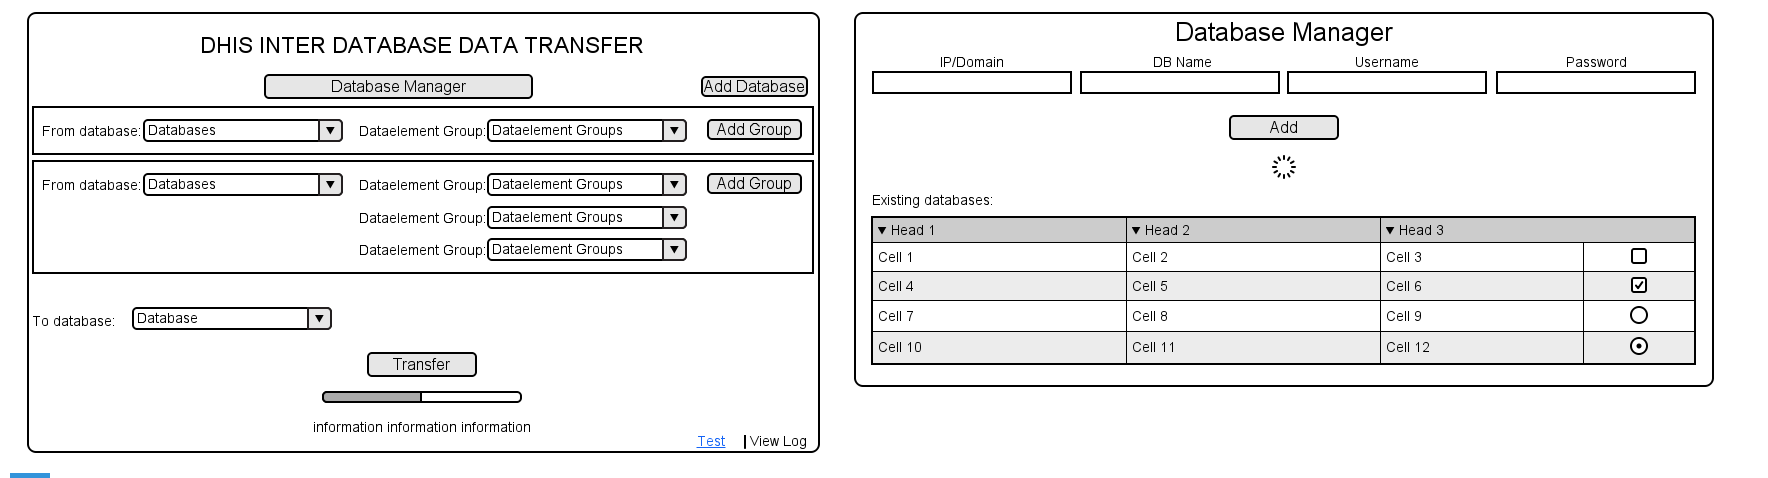
\includegraphics[width="15cm"]{appendix/images/mockup}
I started programming the GUI while Simen took care of the database.
Here the complications startet. We need a way to push datagroups into the other DHIS2 instance.
The web API does not support this.
So in order to do this we have to directly access the database. 
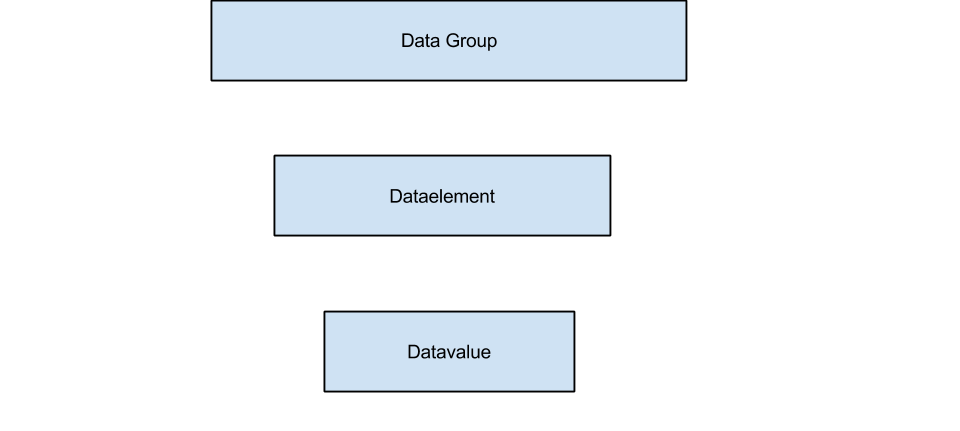
\includegraphics[width="15cm"]{appendix/images/datagroup}
The datagroup consists of several dataelements and a dataelement consists of a datavalue in DHIS2.
In the database it is a different story. There are alot of dependencies. So just pushing everything in would not work.
A problem is that groups, dataelements and datavalues may be there already. Also there is no way that the data is from one DHIS2 instance can identify the same data in another DHIS2 instance. We then thought of a way to handle this. 
Make codes that are equal cross instances and this way make comparison possible.
Dependencies in the database made this not so straight forward. There is a lot of dependencies in the target database that needs to be updateted when introducing new dataelements. I think this was solvable with a recursive algorithm. Simen did not like this. It seems that poking around in a database is not very popular. 
